\documentclass{beamer}

%\documentclass[handout]{beamer}
 
\usepackage[utf8]{inputenc}
\usepackage{graphicx}
\usepackage{wrapfig}
\usepackage{lipsum}
\usepackage{hyperref}
\usepackage{tabularx}
\usepackage{amsmath}
\usepackage{enumerate}
\usepackage[utf8]{inputenc}
\usepackage{tikz}
\usepackage{circuitikz}
\usepackage{xcolor}

\usepackage{pgfpages}

\mode<handout>{%
    \pgfpagesuselayout{4 on 1}[letter] 
    \setbeameroption{show notes}
}

\renewcommand{\vec}[1]{\mathbf{#1}} % Display vectors as boldface %

\let\oldhat\hat   % Also display hats as boldface
\renewcommand{\hat}[1]{\oldhat{\mathbf{#1}}} % Also display hats as boldface
 
%Information to be included in the title page:
\title{Physics 231}
\subtitle{Lecture 4: Op Amps II}
\author{Eric Landahl}
\institute{DePaul University Physics Department}
 
\begin{document}
 
\frame{\titlepage}

\begin{frame}
\frametitle{Table of Contents}
\tableofcontents
\end{frame}}
%%%%%%%%%%%%%%%%%%%%
\section{The Op-Amp Golden Rules}
%%%%%%%%%%%%%%%%%%%%
\begin{frame}{\secname : \subsecname}
    \large The input leads draw no current \\
    \normalsize \emph{High input resistance} \\
    \vspace{0.5 cm} \\
    \large The output can produce enough current to drive any load \\
    \normalsize \emph{Low output resistance} \\
        \vspace{0.5 cm} \\
    \large The output output tries to make the input voltages the same \\
    \normalsize \emph{Operational amplifiers are usually used with feedback}
\end{frame}
%%%%%%%%%%%%%%%%%%%%
\section{Basic Op-Amp Circuits}
%%%%%%%%%%%%%%%%%%%%
\subsection{Follower/Buffer}
%%%%%%%%%%%%%%%%%%%%
\begin{frame}{\secname : \subsecname}
    \begin{equation*}
        V_{out} = V_{in}
    \end{equation*}
    \begin{figure}
    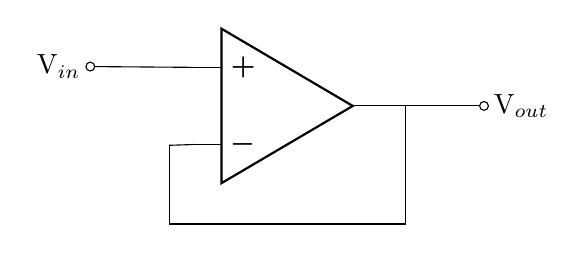
\begin{tikzpicture}
        % Matchmaker
        \draw (6.5,8) node[op amp,yscale=-1](opamp1) {};
        \draw (opamp1.+) to[short,-o] (4,8.5);
        \draw (opamp1.-) to[short,-] (5,7.5);
        \draw (opamp1.out) to[short,-o] (9,8);
        \draw (5,7.5) -- (5,6.5) -- (8,6.5) -- (8,8);
        \draw (4,8.5) node[anchor=east] {V$_{in}$};
        \draw (9,8) node[anchor=west] {V$_{out}$};
    \end{tikzpicture}
    \end{figure}
    \vspace{0.5 cm} \\
    \underline{Task:} Make a follower that buffers negative voltages as well using an LM 741 op-amp.
\end{frame}
%%%%%%%%%%%%%%%%%%%%
\subsection{Comparator}
%%%%%%%%%%%%%%%%%%%%
\begin{frame}{\secname : \subsecname}
\begin{equation*}
  V_{out} \rightarrow  \begin{cases}
    HIGH, & \text{if $V_{in}>V_{ref}$}.\\
    LOW, & \text{if $V_{in}<V_{ref}$}.
  \end{cases}
\end{equation*}
    \begin{figure}
    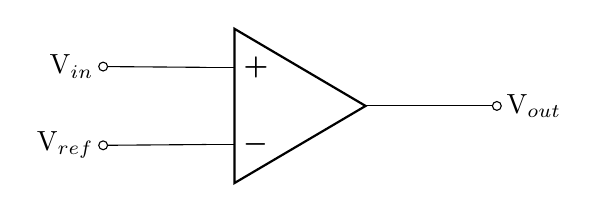
\begin{tikzpicture}
        % Matchmaker
        \draw (6.5,8) node[op amp,yscale=-1](opamp1) {};
        \draw (opamp1.+) to[short,-o] (4,8.5);
        \draw (opamp1.-) to[short,-o] (4,7.5);
        \draw (opamp1.out) to[short,-o] (9,8);
        \draw (4,8.5) node[anchor=east] {V$_{in}$};
        \draw (4,7.5) node[anchor=east] {V$_{ref}$};
        \draw (9,8) node[anchor=west] {V$_{out}$};
    \end{tikzpicture}
    \end{figure}    
    \vspace{0.5 cm} \\
    \underline{Task:} Make an comparator that outputs HIGH when $V_{in}>V_{ref}$.  Set $V_{in}$ using a potentiometer. 
\end{frame}
%%%%%%%%%%%%%%%%%%%%
\subsection{Amplifier (non-inverting)}
%%%%%%%%%%%%%%%%%%%%
\begin{frame}{\secname : \subsecname}
\begin{equation*}
  V_{out} = \left( 1 + \dfrac{R_1}{R_2} \right) V_{in}
\end{equation*}
    \begin{figure}
    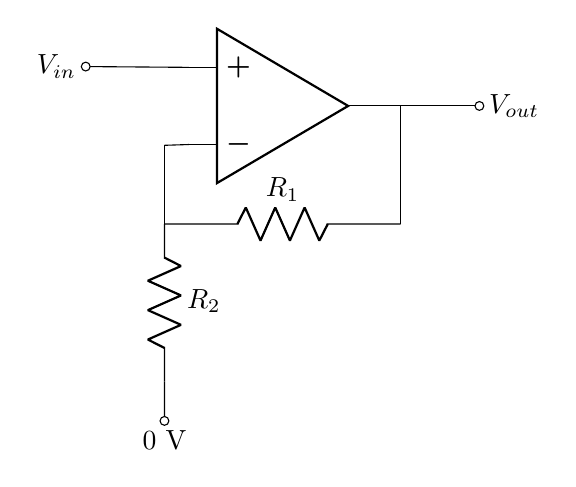
\begin{tikzpicture}
        \draw (6.5,8) node[op amp,yscale=-1](opamp1) {};
        \draw (opamp1.+) to[short,-o] (4,8.5);
        \draw (opamp1.-) to[short,-] (5,7.5);
        \draw (opamp1.out) to[short,-o] (9,8);
        \draw (5,7.5) -- (5,6.5);
        \draw (5,6.5) to[R=$R_1$] (8,6.5); 
        \draw (8,6.5) -- (8,8);
        \draw (5,6.5) to[R=$R_2$] (5,4.5);
        \draw (5,4.5) to[short,-o] (5,4);
        \draw (5,4) node[anchor=north] {0 V};
        \draw (4,8.5) node[anchor=east] {$V_{in}$};
        \draw (9,8) node[anchor=west] {$V_{out}$};
    \end{tikzpicture}
    \end{figure}
    \underline{Task:} Derive the gain equation for this amplifier. \\ \emph{Hint: Adapt the voltage divider equation.}
\end{frame}
%%%%%%%%%%%%%%%%%%%%
\subsection{Amplifier (inverting)}
%%%%%%%%%%%%%%%%%%%%
\begin{frame}{\secname : \subsecname}
    \begin{figure}
    \begin{tikzpicture}
        \draw (6.5,8) node[op amp,yscale=-1](opamp1) {};
        \draw (opamp1.+) to[short,-] (5,8.5);
        \draw (opamp1.-) to[short,-] (5,7.5);
        \draw (opamp1.out) to[short,-o] (9,8);
        \draw (5,8.5) -- (5,9.5);
        \draw (5,9.5) to[R=$R_1$] (8,9.5); 
        \draw (8,9.5) -- (8,8);
        \draw (3,8.5) to[R=$R_2$] (5,8.5);
        \draw (3,8.5) to[short,-o] (2.5,8.5);
        \draw (5,7.5) to[short,-o] (5,6);
        \draw (5,6) node[anchor=north] {0 V};
        \draw (2.5,8.5) node[anchor=east] {$V_{in}$};
        \draw (9,8) node[anchor=west] {$V_{out}$};
    \end{tikzpicture}
    \end{figure}
    \underline{Task:} Derive the gain equation for this amplifier.  Build and test it.  What might this be used for?  What is a disadvantage?
\end{frame}
%%%%%%%%%%%%%%%%%%%%
\subsection{Differential Amplifier}
%%%%%%%%%%%%%%%%%%%%
\begin{frame}{\secname : \subsecname}
    \begin{equation*}
        V_{out}= \dfrac{R_1}{R_2} \left( V_2 - V_1 \right)
    \end{equation*}
    \begin{figure}
    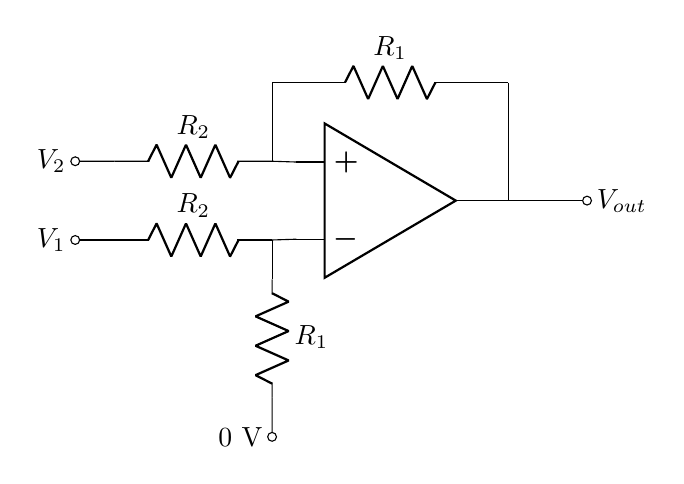
\begin{tikzpicture}
        \draw (6.5,8) node[op amp,yscale=-1](opamp1) {};
        \draw (opamp1.+) to[short,-] (5,8.5);
        \draw (opamp1.-) to[short,-] (5,7.5);
        \draw (opamp1.out) to[short,-o] (9,8);
        \draw (5,8.5) -- (5,9.5);
        \draw (5,9.5) to[R=$R_1$] (8,9.5); 
        \draw (8,9.5) -- (8,8);
        \draw (3,8.5) to[R=$R_2$] (5,8.5);
        \draw (3,8.5) to[short,-o] (2.5,8.5);
        \draw (3,7.5) to[R=$R_2$] (5,7.5);
        \draw (3,7.5) to[short,-o] (2.5,7.5);
        \draw (5,7.5) -- (5,7);
        \draw (5,7) to[R=$R_1$] (5,5.5);
        \draw (5,5.5) to[short,-o] (5,5);
        \draw (5,5) node[anchor=east] {0 V};
        \draw (2.5,7.5) node[anchor=east] {$V_{1}$};
        \draw (2.5,8.5) node[anchor=east] {$V_{2}$};
        \draw (9,8) node[anchor=west] {$V_{out}$};
    \end{tikzpicture}
    \end{figure}
    \underline{Task:} Build and test. \\
    Adapt to amplify small changes around a reference of 2.5 V.
\end{frame}
%%%%%%%%%%%%%%%%%%%%
\section{2 bit Analog-to-Digital Converter (ADC)}
\subsection{}
%%%%%%%%%%%%%%%%%%%%
\begin{frame}{\secname : \subsecname}
    \begin{figure}
    \resizebox{!}{7 cm}{
    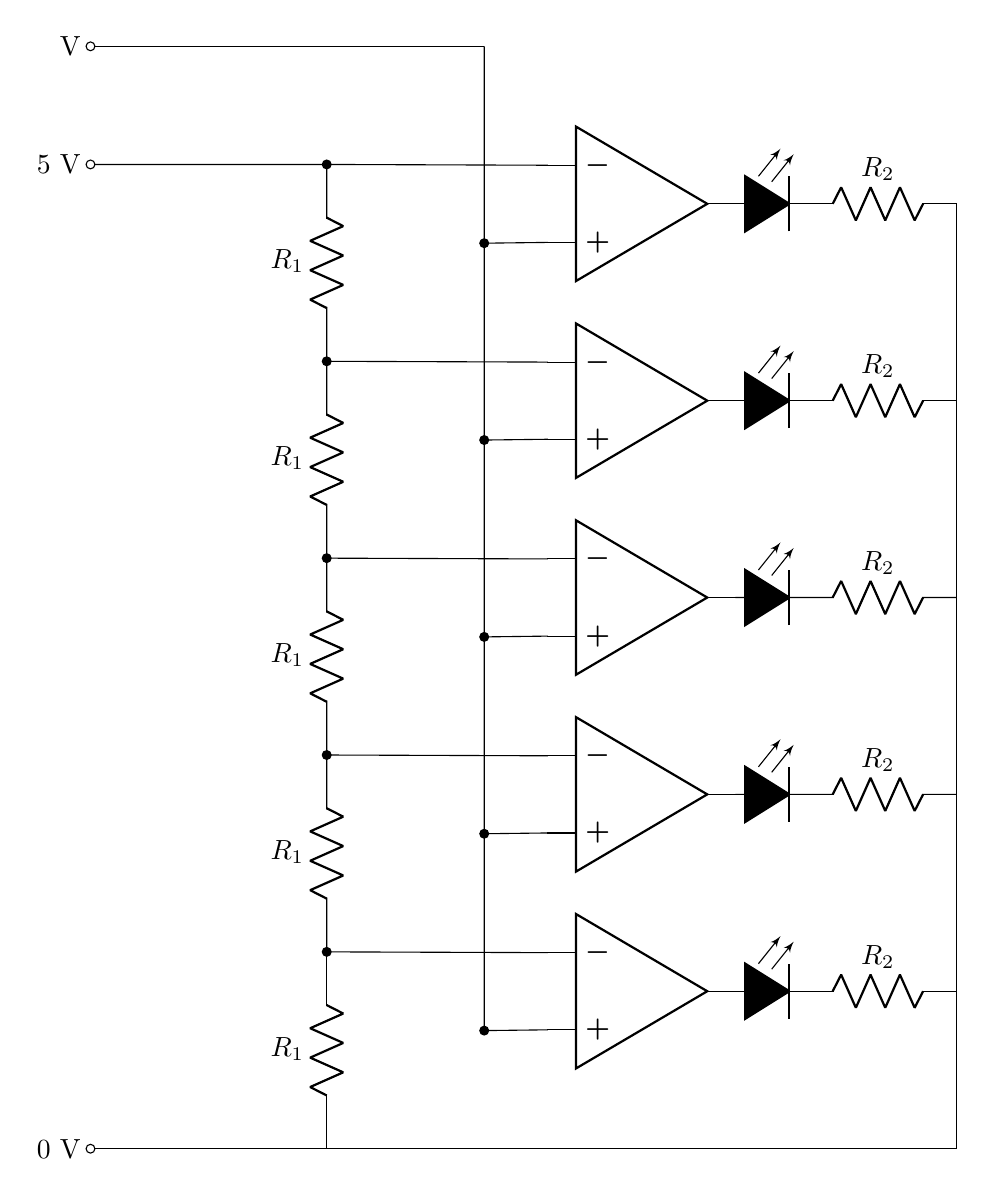
\begin{tikzpicture}

    % Test for > 0 V
     \draw (8,0) node[op amp](opamp1) {}
     (opamp1.+) node[anchor=east] {}
     (opamp1.-) node[anchor=south] {}
     (opamp1.out) node[anchor=north] {};
     \draw (opamp1.-) to[short,-*] (4,0.5)
      to[R=$R_1$] (4,3); 
     \draw (opamp1.+) to[short,-*] (6,-0.5)
      to[short] (6,2);
     \draw (opamp1.out) to[leD*] (10,0)
      to[R=$R_2$] (12,0);

    % Test for > 1 V
     \draw (8,2.5) node[op amp](opamp1) {}
     (opamp1.+) node[anchor=east] {}
     (opamp1.-) node[anchor=south] {}
     (opamp1.out) node[anchor=north] {};
     \draw (opamp1.-) to[short,-*] (4,3)
      to[R=$R_1$] (4,5.5); 
     \draw (opamp1.+) to[short,-*] (6,2)
      to[short] (6,4.5);
     \draw (opamp1.out) to[leD*] (10,2.5)
      to[R=$R_2$] (12,2.5);

     % Test for > 2 V
     \draw (8,5) node[op amp](opamp1) {}
     (opamp1.+) node[anchor=east] {}
     (opamp1.-) node[anchor=south] {}
     (opamp1.out) node[anchor=north] {};
     \draw (opamp1.-) to[short,-*] (4,5.5)
      to[R=$R_1$] (4,8); 
     \draw (opamp1.+) to[short,-*] (6,4.5)
      to[short] (6,7);
     \draw (opamp1.out) to[leD*] (10,5)
  to[R=$R_2$] (12,5);  

     % Test for > 3 V
     \draw (8,7.5) node[op amp](opamp1) {}
     (opamp1.+) node[anchor=east] {}
     (opamp1.-) node[anchor=south] {}
     (opamp1.out) node[anchor=north] {};
     \draw (opamp1.-) to[short,-*] (4,8)
      to[R=$R_1$] (4,10.5); 
     \draw (opamp1.+) to[short,-*] (6,7)
      to[short] (6,9.5);
     \draw (opamp1.out) to[leD*] (10,7.5)
      to[R=$R_2$] (12,7.5);  

      % Test for > 4 V
     \draw (8,10) node[op amp](opamp1) {}
     (opamp1.+) node[anchor=east] {}
     (opamp1.-) node[anchor=south] {}
     (opamp1.out) node[anchor=north] {};
     \draw (opamp1.-) to[short,-*] (4,10.5);
     \draw (opamp1.+) to[short,-*] (6,9.5)
      to[short] (6,12);
     \draw (opamp1.out) to[leD*] (10,10)
      to[R=$R_2$] (12,10);  

     \draw (4,10.5) to[short,-o] (1,10.5); % Connect to 5 V DC
     \draw (1,10.5) node[anchor=east] {5 V};
     \draw (6,12) to[short,-o] (1,12); % Connect to unknown voltage
     \draw (1,12) node[anchor=east] {V};
     
     \draw (4,-2) to[R=$R_1$] (4,0.5);
     \draw (4,-2) to[short,-o] (1,-2); % Connect to common 
     
     %ground reference
     \draw (1,-2) node[anchor=east] {0 V};
     
     % Connect LEDs to ground
     \draw (12,10) -- (12,-2);
     \draw (12,-2) -- (4,-2);

    \end{tikzpicture}
    }
\end{figure}
%    \underline{Task:} Build, test, and explain. 
How would you choose appropriate $R_1$ and $R_2$?\\
%    Modify to be an Arduino input: Write V in binary, and decimal.
    

\end{frame}
\end{document}